\section{Erwartetes Ergebnis} 

Unser geplantes Spiel Layout sieht vor, dass jeder Client eigentlich nur seine bis zu 6 Nachbarn kennt. Der rest des Spiels ist ihm nicht direkt bekannt. Dadurch wollen wir erreichen, dass der Workload lokal in einer kleinen Gruppe bleibt und sich nicht aufs komplette System exponentiell auswirkt.

Figure~\ref{ergebnisspiellayout} zeigt wie genau sich der Client verhält und was genau er überhaupt wahr nimmt.
Er bekommt vom Server alle nötigen inputs und versucht danach auf den Stapeln von sich selbst und den Stapeln seiner Nachbarn seine Karten los zu werden. Gelingt ihm dies nicht geht er weiter zur nächsten Karte, bis es ihm gelingt. Wir hatten uns überlegt zuerst zu prüfen ob auf einem Nachbar Stapel eine Karte gelegt werden könnte und es dann zu tun, sind aber von diesem Ansatz wieder weggekommen, weil in der Zwischenzeit bereits andere Clients dem Client sehr wahrscheinlich zuvorkommen würden und damit viele versuche eine Karte zu legen sowieso misslingen wird. Ob wird nun ständig versuchen eine Karte zu legen oder ob wir ständig Prüfen ob eine Karte legbar ist und danach versuchen die Karte zu legen kommt fast auf das selbe hinaus.


\begin{figure}[hbt]
  \centering
  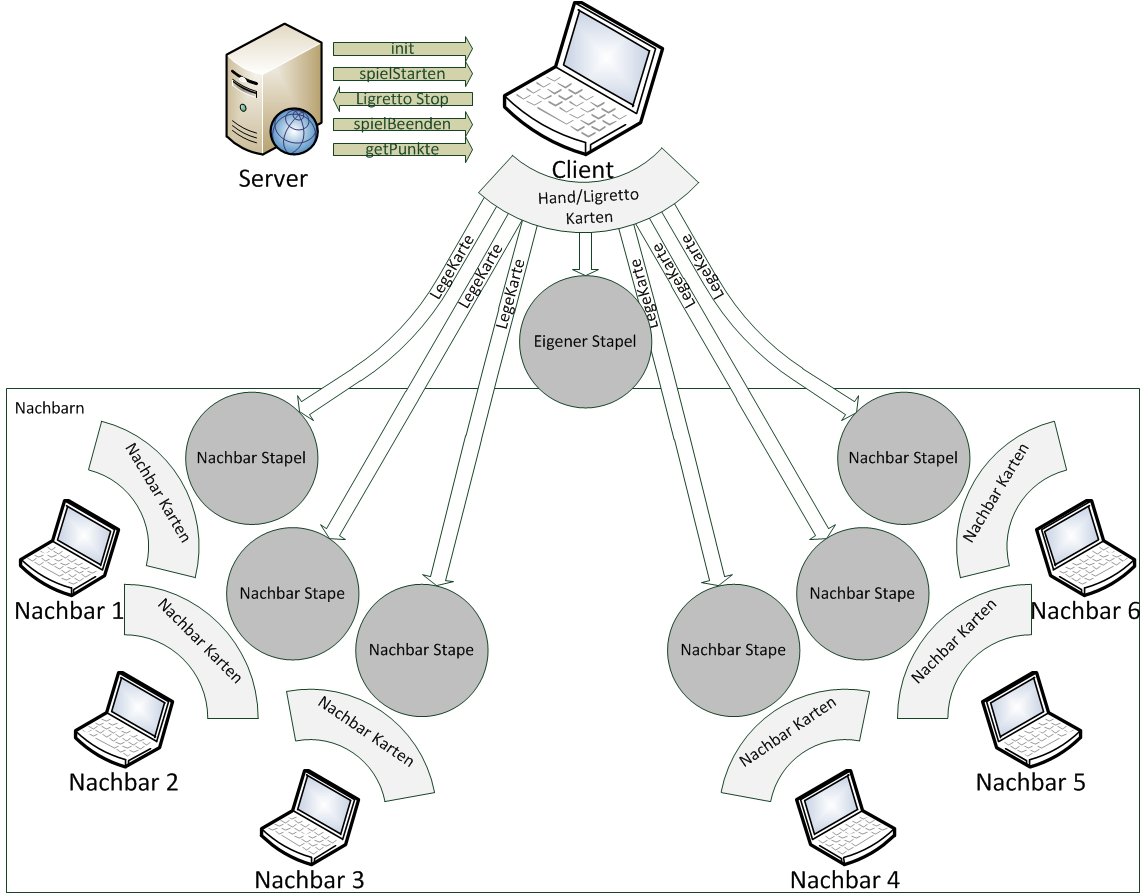
\includegraphics[width=19\textwidth,angle=0]{graphics/SpielLayout.png}
  \caption{Spiel aus Client-Sicht \hfill{} }
  \label{ergebnisspiellayout}
 \end{figure}

\subsection{Auswirkungen bei starker Skallierung}




















%Ausarbeitung / Darstellung (0 Punkte / max. 2 Bonuspunkte)
%    - Grafiken Zusatzpunkte erhalten Sie hier für eine gute Ausarbeitung wie spezifische Grafiken / Ablaufdiagramme etc. max. 2 Punkte. 0 Punkte ist 'normal', 1/2 Punkt für 1-2 spezifische nutzbringende Grafiken, 1 Punkte für ausführliches Nutzen von Grafiken.
%    - Detaillierungsgrad: Je nach Tiefe und Detaillierungsgrad Ihrer Ausarbeitung können Sie bis zu einem Zusatzpunkt holen (0=normal, 1/2=detailliert, 1=sehr detailliert)